\qrchapterstar{https://forgottenpillar.com/rsc/en-fp-appendix}{Appendix} \label{chap:appendix}


\qrchapterstar{https://forgottenpillar.com/rsc/en-fp-appendix}{Nyongeza} \label{chap:appendix}


\addcontentsline{toc}{chapter}{Appendix}


\addcontentsline{toc}{chapter}{Nyongeza}


\section*{The Fundamental Principles 1889}


\section*{Kanuni za Msingi 1889}


As elsewhere stated, Seventh-day Adventists have no creed but the Bible; but they hold to certain well-defined points of faith for which they feel prepared to give a reason “to every man that asketh” them. The following propositions may be taken as a summary of the principal features of their religious faith, upon which there is, so far as we know, entire unanimity throughout the body. They believe,—


Kama ilivyoelezwa mahali pengine, Waadventista Wasabato hawana imani ila Biblia; lakini wanashikilia mambo fulani ya imani yaliyofafanuliwa vizuri ambayo wanahisi kuwa tayari kutoa sababu “kwa kila mtu awaulizaye”. Mapendekezo yafuatayo yanaweza kuchukuliwa kama muhtasari wa sifa kuu za imani yao ya kidini, ambayo juu yake kuna, kama tujuavyo, umoja mzima katika mwili wote. Wanaamini,—


\lettrine{I.} That there is one God, a personal, spiritual being, the creator of all things, omnipotent, omniscient, and eternal; infinite in wisdom, holiness, justice, goodness, truth, and mercy; unchangeable, and everywhere present by his representative, the Holy Spirit. Psalm 139:7.


\lettrine{I.} Kwamba kuna Mungu mmoja huluki binafsi wa kiroho, Muumba wa vitu vyote, muweza wa yote, mwenye kujua yote, na wa milele; asiye na kikomo katika hekima, utakatifu, haki, wema, ukweli, na rehema; asiyebadilika, na kila mahali akiwepo kwa mwakilishi wake, Roho Mtakatifu. Zaburi 139:7.


\lettrine{II.} That there is one Lord Jesus Christ, the Son of the Eternal Father, the one by whom he created all things, and by whom they do consist; that he took on him the nature of the seed of Abraham for the redemption of our fallen race; that he dwelt among men, full of grace and truth, lived our example, died our sacrifice, was raised for our justification, ascended on high to be our only mediator in the sanctuary in heaven, where, through the merits of his shed blood, he secures the pardon and forgiveness of the sins of all those who penitently come to him; and as the closing portion of his work as priest, before he takes his throne as king, he will make the great atonement for the sins of all such, and their sins will then be blotted out (Acts 3:19) and borne away from the sanctuary, as shown in the service of the Levitical priesthood, which foreshadowed and prefigured the ministry of our Lord in heaven. See Leviticus 16; Hebrews 8:4, 5; 9:6, 7; etc.


\lettrine{II.} Kwamba kuna Bwana mmoja Yesu Kristo, Mwana wa Baba wa Milele, ambaye kwa yeye yeye aliumba vitu vyote, na kwa yeye vinadumishwa; kwamba alichukua asili ya mbegu ya Ibrahimu kwa ukombozi wa kizazi chetu kilichoanguka; kwamba alikaa kati ya watu, amejaa neema na ukweli, aliishi kielelezo chetu, alikufa dhabihu yetu, aliinuliwa kwa ajili ya kuhesabiwa haki kwetu, alipaa juu kuwa mpatanishi wetu wa pekee katika patakatifu pa mbinguni, ambapo, kwa wema wa damu yake iliyomwagika, anapata msamaha na msamaha wa dhambi za wale wote wanaokuja kwake kwa toba; na kama sehemu ya mwisho ya kazi yake ya ukuhani, kabla hajachukua kiti chake cha enzi kama mfalme, yeye atafanya upatanisho mkubwa kwa dhambi za wote hao, na dhambi zao zitafutwa (Matendo 3:19) na kuchukuliwa mbali na patakatifu, kama inavyoonyeshwa katika utumishi wa ukuhani wa Walawi, ambao ulitangulia na kufananisha huduma ya Bwana wetu aliye mbinguni. Tazama Mambo ya Walawi 16; Waebrania 8:4, 5; 9:6, 7; na kadhalika.


\lettrine{III.} That the Holy Scriptures of the Old and New Testaments were given by inspiration of God, contain a full revelation of his will to man, and are the only infallible rule of faith and practice.


\lettrine{III.} Kwamba Maandiko Matakatifu ya Agano la Kale na Agano Jipya yalitolewa kwa uvuvio wa Mungu, yana ufunuo kamili ya mapenzi yake kwa mwanadamu, na ndiyo kanuni pekee isiyoweza kukosea ya imani na mazoezi.


\lettrine{IV.} That baptism is an ordinance of the Christian church, to follow faith and repentance,—an ordinance by which we commemorate the resurrection of Christ, as by this act we show our faith in his burial and resurrection, and through that, in the resurrection of all the saints at the last day; and that no other mode more fitly represents these facts than that which the Scriptures prescribe, namely, immersion. Romans 6:3-5; Colossians 2:12.


\lettrine{IV.} Kwamba Ubatizo ni agizo la kanisa la Kikristo, kufuata imani na toba—agizo ambalo kwalo tunaadhimisha ufufuo wa Kristo, kwani kwa tendo hili tunaonyesha Imani yetu katika kuzikwa na kufufuka kwake, na kwa njia hiyo, katika ufufuo wa watakatifu wote katika ufufuo siku ya mwisho; na kwamba hakuna hali nyingine inayowakilisha ukweli huu kwa ufaafu zaidi ya ile ambayo Maandiko yanaagiza, yaani, kuzamishwa. Warumi 6:3-5; Wakolosai 2:12.


\lettrine{V.} That the new birth comprises the entire change necessary to fit us for the kingdom of God, and consists of two parts; First, a moral change wrought by conversion and a Christian life (John 3:3, 5); second, a physical change at the second coming of Christ, whereby, if dead, we are raised incorruptible, and if living, are changed to immortality in a moment, in the twinkling of an eye. Luke 20:36; 1 Corinthians 15:51, 52.


\lettrine{V.} Kwamba kuzaliwa upya kunajumuisha mabadiliko yote muhimu ili kutufaa kwa ufalme wa Mungu; na lina sehemu mbili; Kwanza, mabadiliko ya kimaadili yanayoletwa na wongofu na maisha ya Kikristo (Yohana 3:3, 5); pili, mabadiliko ya kimwili katika ujio wa pili wa Kristo, ambapo, ikiwa tumekufa, tunafufuliwa bila kuharibika, na ikiwa tunaishi, tunabadilishwa kuwa kutokufa kwa dakika moja, ndani kufumba na kufumbua. Luka 20:36; 1 Wakorintho 15:51, 52.


\lettrine{VI.} That prophecy is a part of God’s revelation to man; that it is included in that Scripture which is profitable for instruction (2 Timothy 3:16); that it is designed for us and our children (Deuteronomy 29:29); that so far from being enshrouded in impenetrable mystery, it is that which especially constitutes the word of God a lamp to our feet and a light to our path (Psalm 119:105; 2 Peter 1:19); that a blessing is pronounced upon those who study it (Revelation 1:1-3); and that, consequently, it is to be understood by the people of God sufficiently to show them their position in the world’s history and the special duties required at their hands.


\lettrine{VI.} Kwamba Unabii ni sehemu ya ufunuo wa Mungu kwa mwanadamu; kwamba imejumuishwa katika Maandiko hayo ambayo yafaa kwa mafundisho (2 Timotheo 3:16); kwamba imeundwa kwa ajili yetu na watoto wetu (Kumbukumbu la Torati 29:29); kwamba mbali na kugubikwa na fumbo lisilopenyeka, ni hilo ambayo hasa hufanya neno la Mungu kuwa taa ya miguu yetu na mwanga wa njia yetu (Zaburi 119:105; 2 Petro 1:19); kwamba baraka inatamkwa juu ya wale wanaoisoma (Ufunuo 1:1-3); na kwamba, kwa hivyo, inapaswa kueleweka na watu wa Mungu vya kutosha kuwaonyesha msimamo wao katika historia ya ulimwengu na majukumu maalum yanayohitajika mikononi mwao.


\lettrine{VII.} That the world’s history from specified dates in the past, the rise and fall of empires, and the chronological succession of events down to the setting up of God’s everlasting kingdom, are outlined in numerous great chains of prophecy; and that these prophecies are now all fulfilled except the closing scenes.


\lettrine{VII.} Kwamba historia ya dunia kutoka tarehe maalum katika siku za nyuma, kupanda na kuanguka kwa himaya, na mfululizo wa matukio hadi kusimamishwa kwa ufalme wa milele wa Mungu, yameainishwa katika minyororo mingi mikuu ya unabii; na kwamba unabii huu wote sasa umetimia isipokuwa matukio ya kufunga.


\lettrine{VIII.} That the doctrine of the world’s conversion and a temporal millennium is a fable of these last days, calculated to lull men into a state of carnal security, and cause them to be overtaken by the great day of the Lord as by a thief in the night (1 Thessalonians 5:3); that the second coming of Christ is to precede, not follow, the millennium; for until the Lord appears, the papal power, with all its abominations, is to continue (2 Thessalonians 2:8), the wheat and tares grow together (Matthew 13:29, 30, 39), and evil men and seducers wax worse and worse, as the word of God declares. 2 Timothy 3:1, 13.


\lettrine{VIII.} Kwamba fundisho la uongofu wa ulimwengu na milenia ya muda ni hekaya ya siku hizi za mwisho, zilizohesabiwa kuwarubuni watu katika hali ya usalama wa kimwili, na kuwafanya kupatikana na siku ile kuu ya Bwana kama vile mwivi usiku (1 Wathesalonike 5:3); hiyo ujio wa pili wa Kristo ni kutangulia, si kufuata, milenia; kwa maana mpaka Bwana aonekane, mamlaka ya upapa, pamoja na machukizo yake yote, yataendelea (2 Wathesalonike 2:8), ngano na magugu hukua pamoja (Mathayo 13:29, 30, 39), na watu waovu na wadanganyi huzidi kuwa mbaya zaidi na mbaya zaidi, kama neno la Mungu linavyotangaza. 2 Timotheo 3:1, 13.


\lettrine{IX.} That the mistake of Adventists in 1844 pertained to the nature of the event then to transpire, not to the time; that no prophetic period is given to reach to the second advent, but that the longest one, the two thousand and three hundred days of Daniel 8:14, terminated in 1844, and brought us to an event called the cleansing of the sanctuary.


\lettrine{IX.} Kwamba kosa la Waadventista mwaka 1844 lilihusu asili ya tukio basi kwa kutokea, si kwa wakati; kwamba hakuna kipindi cha kinabii kinachotolewa kufikia ujio wa pili, bali kwamba ile ndefu zaidi, zile siku elfu mbili na mia tatu za Danieli 8:14, ziliisha 1844, na kutuleta kwenye tukio linaloitwa utakaso wa patakatifu.


\lettrine{X.} That the sanctuary of the new covenant is the tabernacle of God in heaven, of which Paul speaks in Hebrews 8 and onward, and of which our Lord, as great high priest, is minister; that this sanctuary is the antitype of the Mosaic tabernacle, and that the priestly work of our Lord, connected therewith, is the antitype of the work of the Jewish priests of the former dispensation (Hebrews 8:1-5, etc.); that this, and not the earth, is the sanctuary to be cleansed at the end of the two thousand and three hundred days, what is termed its cleansing being in this case, as in the type, simply the entrance of the high priest into the most holy place, to finish the round of service connected therewith, by making the atonement and removing from the sanctuary the sins which had been transferred to it by means of the ministration in the first apartment (Leviticus 16; Hebrews 9:22, 23); and that this work in the antitype, beginning in 1844, consists in actually blotting out the sins of believers (Acts 3:19), and occupies a brief but indefinite space of time, at the conclusion of which the work of mercy for the world will be finished, and the second advent of Christ will take place.


\lettrine{X.} Kwamba patakatifu pa agano jipya ni maskani ya Mungu mbinguni, ambayo Paulo hunena katika Waebrania 8 na kuendelea, na ambayo Bwana wetu, aliye kuhani mkuu, anahudumu; kwamba patakatifu hapa ni mfano wa hema ya Musa, na kwamba kazi ya ukuhani wa Bwana wetu, aliyeunganishwa nayo, ndiye mfano wa kazi ya makuhani wa Kiyahudi wa kipindi cha zamani (Waebrania 8:1-5, nk.); kwamba hii, na si dunia, ni patakatifu pa kutakaswa mwishoni mwa zile siku elfu mbili na mia tatu, zile zinazoitwa utakaso zake kuwa katika kesi hii, kama mfano, kuingia tu kwa kuhani mkuu katika mahali patakatifu pa patakatifu, ili kumalizia duru ya huduma iliyounganishwa nayo, kwa kufanya upatanisho na kuondoa kutoka kwa Patakatifu dhambi zilizohamishwa kwake kwa njia ya huduma katika chumba cha kwanza (Mambo ya Walawi 16; Waebrania 9:22, 23); na kwamba kazi hii katika mfano, kuanzia 1844, inajumuisha kufuta dhambi za waumini (Matendo 3:19), na inachukua muda mfupi lakini usio na kipimo wa wakati, katika hitimisho ambalo kazi ya rehema kwa ulimwengu itakamilika, na ujio wa pili wa Kristo utatokea.


\lettrine{XI.} That God’s moral requirements are the same upon all men in all dispensations; that these are summarily contained in the commandments spoken by Jehovah from Sinai, engraven on the tables of stone, and deposited in the ark, which was in consequence called the “ark of the covenant,” or testament (Numbers 10:33; Hebrews 9:4, etc.); that this law is immutable and perpetual, being a transcript of the tables deposited in the ark in the true sanctuary on high, which is also, for the same reason, called the ark of God’s testament; for under the sounding of the seventh trumpet we are told that “the temple of God was opened in heaven, and there was seen in his temple the ark of his testament.” Revelation 11:19.


\lettrine{XI.} Kwamba matakwa ya Mungu ya kimaadili ni sawa kwa wanadamu wote katika vipindi vyote; Kwamba haya yamo katika amri zilizonenwa na Yehova kutoka Sinai, zilizochongwa juu ya mbao za mawe, na kuwekwa katika safina, ambayo ilikuwa katika matokeo iliitwa “sanduku la agano,” au agano (Hesabu 10:33; Waebrania 9:4, nk.); kwamba sheria hii isiyobadilika na ya kudumu, ikiwa ni nakala ya meza zilizowekwa ndani ya safina katika patakatifu pa kweli palipo juu, ambapo pia, kwa sababu iyo hiyo, huitwa sanduku la agano la Mungu; wakati wa kupigwa kwa baragumu ya saba tunaambiwa kwamba “hekalu la Mungu likafunguliwa mbinguni, na sanduku la agano lake lilionekana katika hekalu lake.” Ufunuo 11:19.


\lettrine{XII.} That the fourth commandment of this law requires that we devote the seventh day of each week, commonly called Saturday, to abstinence from our own labor, and to the performance of sacred and religious duties; that this is the only weekly Sabbath known to the Bible, being the day that was set apart before Paradise was lost (Genesis 2:2, 3), and which will be observed in Paradise restored (Isaiah 66:22, 23); that the facts upon which the Sabbath institution is based confine it to the seventh day, as they are not true of any other day; and that the terms Jewish Sabbath, as applied to the seventh day, and Christian Sabbath, as applied to the first day of the week, are names of human invention, unscriptural in fact, and false in meaning.


\lettrine{XII.} Kwamba amri ya nne ya sheria hii inatutaka tuiweke siku ya saba ya kila juma, inayojulikana sana kuwa Jumamosi, kujiepusha na kazi yetu wenyewe, na kwa utekelezaji wa majukumu matakatifu na ya kidini; kwamba hii ndiyo Sabato pekee ya kila juma inayojulikana kwa Biblia, ikiwa ni siku iliyotengwa kabla ya Paradiso kupotea (Mwanzo 2:2, 3), na ambayo itaadhimishwa katika Paradiso iliyorudishwa (Isaya 66:22, 23); kwamba ukweli kuhusu Maadhimisho ya Sabato ni msingi wa kuifungia siku ya saba, kwa kuwa si kweli kwa siku yoyote nyingine; na kwamba maneno Sabato ya Kiyahudi, kama inavyotumika kwa siku ya saba, na Sabato ya Mkristo, kama inavyotumiwa kwa siku ya kwanza ya juma, ni majina ya uvumbuzi wa wanadamu, yasiyo ya kimaandiko kwa kweli, na maana ya uwongo.


\lettrine{XIII.} That as the man of sin, the papacy, has thought to change times and laws (the law of God, Daniel 7:25), and has misled almost all Christendom in regard to the fourth commandment, we find a prophecy of a reform in this respect to be wrought among believers just before the coming of Christ. Isaiah 56:1, 2; 1 Peter 1:5; Revelation 14:12, etc.


\lettrine{XIII.} Kwamba kama mtu wa dhambi, upapa, amefikiria kubadili nyakati na sheria (sheria ya Mungu, Danieli 7:25), na amepotosha karibu Jumuiya ya Wakristo yote kuhusiana na ile amri ya nne, tunapata unabii wa mageuzi katika suala hili kufanywa kati ya waumini kabla tu ya kuja kwa Kristo. Isaya 56:1, 2; 1 Petro 1:5; Ufunuo 14:12, nk.


\lettrine{XIV.} That the followers of Christ should be a peculiar people, not following the maxims, nor conforming to the ways, of the world; not loving its pleasures nor countenancing its follies; inasmuch as the apostle says that “whosoever therefore will be” in this sense, “a friend of the world, is the enemy of God” (James 4:4); and Christ says that we cannot have two masters, or, at the same time, serve God and mammon. Matthew 6:24.


\lettrine{XIV.} Kwamba wafuasi wa Kristo wanapaswa kuwa watu wa kipekee, si kufuata kanuni, wala wakipatana na njia, za ulimwengu; kutopenda anasa zake wala kukabili upumbavu wake; kama vile mtume asemavyo kwamba “yeyote atakaye kuwa” katika maana hii, “rafiki wa ulimwengu ni adui wa Mungu” (Yakobo 4:4); na Kristo anasema kwamba hatuwezi kuwa na mabwana wawili, au, wakati huo huo, kumtumikia Mungu na mali. Mathayo 6:24.


\lettrine{XV.} That the Scriptures insist upon plainness and modesty of attire as a prominent mark of discipleship in those who profess to be the followers of Him who was, “meek and lowly in heart,” that the wearing of gold, pearls, and costly array, or anything designed merely to adorn the person and foster the pride of the natural heart, is to be discarded, according to such scriptures as 1 Timothy 2:9, 10; 1 Peter 3:3, 4.


\lettrine{XV.} Kwamba Maandiko yanasisitiza juu ya uwazi na staha ya mavazi kama alama kuu ya ufuasi kati ya wale wanaodai kuwa wafuasi wa Yeye ambaye alikuwa, “mpole na mnyenyekevu katika moyo,” kwamba kuvaa dhahabu, lulu, na mavazi ya bei ghali, au chochote kilichobuniwa tu kupamba mtu na kukuza kiburi cha moyo wa asili, ni kutupwa, kulingana na maandiko kama vile 1 Timotheo 2:9, 10; 1 Petro 3:3, 4.


\lettrine{XVI.} That means for the support of evangelical work among men should be contributed from love to God and love of souls, not raised by church lotteries, or occasions designed to contribute to the fun-loving, appetite-indulging propensities of the sinner, such as fairs, festivals, oyster suppers, tea, broom, donkey, and crazy socials, etc., which are a disgrace to the professed church of Christ; that the proportion of one’s income required in former dispensation can be no less under the gospel; that it is the same as Abraham (whose children we are, if we are Christ’s, Galatians 3:29) paid to Melchisedec (type of Christ) when he gave him a tenth of all (Hebrews 7:1-4); the title is the Lord’s (Leviticus 27:30); and this tenth of one’s income is also to be supplemented by offerings from those who are able, for the support of the gospel. 2 Corinthians 9:6; Malachi 3:8, 10.


\lettrine{XVI.} Hiyo ina maana kwa ajili ya msaada wa kazi ya kiinjilisti kati ya watu inapaswa kuchangiwa kwa upendo kwa Mungu na upendo wa roho, sio kukuzwa na bahati nasibu ya kanisa, au hafla zilizokusudiwa kuchangia tabia ya kupenda kujifurahisha, na kufurahisha tamaa ya mwenye dhambi, kama vile maonyesho, sherehe, karamu za oyster, chai, ufagio, punda, na jamii za wazimu, n.k., ambazo ni aibu kwa kanisa linalojiita la Kristo; kwamba sehemu ya mapato ya mtu inayohitajika hapo awali maongozi hayawezi kuwa machache chini ya injili; kwamba ni sawa na Ibrahimu (ambaye sisi ni watoto, kama sisi ni wa Kristo, Wagalatia 3:29) tunalipwa kwa Melkizedeki (aina ya Kristo) wakati alimpa sehemu ya kumi ya vitu vyote (Waebrania 7:1-4); cheo ni cha Bwana (Mambo ya Walawi 27:30); na hii sehemu ya kumi ya mapato ya mtu pia inapaswa kuongezwa na matoleo kutoka kwa wale wanaoweza, kwa msaada wa injili. 2 Wakorintho 9:6; Malaki 3:8, 10.


\lettrine{XVII.} That as the natural or carnal heart is at enmity with God and his law, this enmity can be subdued only by a radical transformation of the affections, the exchange of unholy for holy principles; that this transformation follows repentance and faith, is the special work of the Holy Spirit, and constitutes regeneration, or conversion.


\lettrine{XVII.} Kwamba kama vile moyo wa asili au wa kimwili uko katika uadui na Mungu na sheria yake, uadui huu unaweza kutiishwa tu na mabadiliko makubwa ya mapenzi, kubadilishana kanuni yasiyo takatifu kwa matakatifu; kwamba mageuzi haya yanafuata toba na imani, ni kazi maalum ya Roho Mtakatifu, na hujumuisha kuzaliwa upya, au kuongoka.


\lettrine{XVIII.} That as all have violated the law of God, and cannot of themselves render obedience to his just requirements, we are dependent on Christ, first, for justification from our past offenses, and, secondly, for grace whereby to render acceptable obedience to his holy law in time to come.


\lettrine{XVIII.} Kwamba kama wote wamevunja sheria ya Mungu, na hawawezi kwa wao wenyewe kutoa utii kwa matakwa yake ya haki, tunamtegemea Kristo, kwanza, kwa ajili ya kuhesabiwa haki kutokana na makosa yetu ya zamani, na pili, kwa neema ambayo kwayo wanaweza kutoa utii unaokubalika kwa sheria yake takatifu katika wakati ujao.


\lettrine{XIX.} That the Spirit of God was promised to manifest itself in the church through certain gifts, enumerated especially in 1 Corinthians 12 and Ephesians 4; that these gifts are not designed to supersede, or take the place of, the Bible, which is sufficient to make us wise unto salvation, any more than the Bible can take the place of the Holy Spirit; that, in specifying the various channels of its operation, that Spirit has simply made provision for its own existence and presence with the people of God to the end of time, to lead to an understanding of that word which it had inspired, to convince of sin, and to work a transformation in the heart and life; and that those who deny to the Spirit its place and operation, do plainly deny that part of the Bible which assigns to it this work and position.


\lettrine{XIX.} Kwamba Roho wa Mungu aliahidiwa kujidhihirisha ndani ya kanisa kupitia karama Fulani, imeorodheshwa hasa katika 1 Wakorintho 12 na Waefeso 4; kwamba karama hizi sio iliyokusudiwa kuchukua nafasi, au kuchukua mahali pa, Biblia, ambayo inatosha kutufanya tuwe na hekima kwa wokovu, kama vile Biblia haiwezi kuchukua mahali pa Roho Mtakatifu; hivyo, katika kibainisha mikondo mbalimbali ya utendaji wake, Roho huyo ameifanya kwa urahisi uwepo na uwepo wake pamoja na watu wa Mungu hadi mwisho wa nyakati, ili kuongoza kwenye ufahamu wa neno lile ambalo lilikuwa limevuviwa, kusadikisha juu ya dhambi, na kufanya kazi ya mabadiliko katika moyo na maisha; na kwamba wale wanaomkana Roho mahali pake na utendakazi wake, hukataa kwa uwazi ile sehemu ya Biblia ambayo inaipa kazi hii na msimamo huu.


\lettrine{XX.} That God, in accordance with his uniform dealings with the race, sends forth a proclamation of the approach of the second advent of Christ; and that this work is symbolized by the three messages of Revelation 14, the last one bringing to view the work of reform on the law of God, that his people may acquire a complete readiness for that event.


\lettrine{XX.} Kwamba Mungu, kwa mujibu wa shughuli zake sawa na mbio, anatuma tangazo la kukaribia kwa ujio wa pili wa Kristo; na kwamba kazi hii inafananishwa na jumbe tatu za Ufunuo 14, ujumbe wa mwisho unaoleta kutazama kazi ya kurekebisha sheria ya Mungu, ili watu wake wapate kuwa tayari kabisa kwa ajili ya tukio hilo.


\lettrine{XXI.} That the time of the cleansing of the sanctuary (See proposition X.), synchronizing with the time of the proclamation of the third message (Revelation 14:9, 10), is a time of investigative judgment, first, with reference to the dead, and secondly, at the close of probation, with reference to the living, to determine who of the myriads now sleeping in the dust of the earth are worthy of a part in the first resurrection, and who of its living multitudes are worthy of translation,—points which must be determined before the Lord appears.


\lettrine{XXI.} Kwamba wakati wa kutakaswa kwa patakatifu (Angalia pendekezo la X.), linalolingana na wakati wa kutangazwa kwa ujumbe wa tatu (Ufunuo 14:9, 10), ni wakati wa hukumu ya uchunguzi, kwanza, kwa kuzingatia wafu, na pili, mwishoni mwa muda wa majaribio, kwa kurejelea walio hai, ili kubaini ni nani kati ya maelfu ya maelfu ya watu wanaolala ndani ya mavumbi ya nchi wanastahili sehemu katika ufufuo wa kwanza, na ni nani kati ya watu wake walio hai wanastahili kubadilishwa,—mambo ambayo ni lazima yaamuliwe kabla ya Bwana kutokea.


\lettrine{XXII.} That the grave, whether we all tend, expressed by the Hebrew word sheol and the Greek word hades, is a place, or condition, in which there is no work, device, wisdom, nor knowledge. Ecclesiastes 9:10.


\lettrine{XXII.} Kwamba kaburi, kama sisi sote tunaelekea, linaonyeshwa na neno la Kiebrania sheol na Neno la Kigiriki hades, ni mahali, au hali, ambapo hakuna kazi, kifaa, hekima, wala maarifa. Mhubiri 9:10.


\lettrine{XXIII.} That the state to which we are reduced by death is one of silence, inactivity, and entire unconsciousness. Psalm 146:4; Ecclesiastes 9:5, 6; Daniel 12:2.


\lettrine{XXIII.} Kwamba hali ambayo tunapunguzwa na kifo ni ya ukimya, kutofanya kazi, na kupoteza fahamu. Zaburi 146:4; Mhubiri 9:5, 6; Danieli 12:2.


\lettrine{XXIV.} That out of this prison-house of the grave, mankind are to be brought by a bodily resurrection; the righteous having part in the first resurrection, which takes place at the second coming of Christ; the wicked, in the second resurrection, which takes place in a thousand years thereafter. Revelation 20:4-6.


\lettrine{XXIV.} Kwamba kutoka katika gereza hili la kaburi, wanadamu wataletwa kwa ufufuo wa mwili; wenye haki walio na sehemu katika ufufuo wa kwanza, utakaofanyika katika ujio wa pili wa Kristo; waovu, katika ufufuo wa pili, unaofanyika katika miaka elfu baada ya hapo. Ufunuo 20:4-6.


\lettrine{XXV.} That at the last trump, the living righteous are to be changed in a moment, in the twinkling of an eye, and with the risen righteous are to be caught up to meet the Lord in the air, so forever to be with the Lord. 1 Thessalonians 4:16, 17; 1 Corinthians 15:51, 52.


\lettrine{XXV.} Kwamba wakati wa parapanda ya mwisho, wenye haki walio hai watabadilishwa mara moja, katika kupepesa macho, na wenye haki waliofufuka watanyakuliwa ili kumlaki Bwana katika anga, hivyo kuwa na Bwana milele. 1 Wathesalonike 4:16, 17; 1 Wakorintho 15:51, 52.


\lettrine{XXVI.} That these immortalized ones are then taken to heaven, to the New Jerusalem, the Father’s house, in which there are many mansions (John 14:1-3), where they reign with Christ a thousand years, judging the world and fallen angels, that is, apportioning the punishment to be executed upon them at the close of the one thousand years (Revelation 20:4; 1 Corinthians 6:2, 3); that during this time the earth lies in a desolate and chaotic condition (Jeremiah 4:23-27), described, as in the beginning, by the Greek term abussos— “bottom-less pit” (Septuagint of Genesis 1:2); and that here Satan is confined during the thousand years (Revelation 20:1, 2), and here finally destroyed (Revelation 20:10; Malachi 4:1); the theater of the ruin he has wrought in the universe being appropriately made, for a time, his gloomy prison-house, and then the place of his final execution.


\lettrine{XXVI.} Kwamba hawa wasioweza kufa kisha wanachukuliwa kwenda mbinguni, kwenye Yerusalemu Mpya, Nyumba ya Baba, ambamo mna makao mengi (Yohana 14:1-3), ambamo wanatawala naye Kristo miaka elfu, wakihukumu ulimwengu na malaika walioanguka, yaani, kugawanya adhabu itakayotekelezwa juu yao mwishoni mwa ile miaka elfu moja (Ufunuo 20:4; 1 Wakorintho 6:2, 3); kwamba wakati huu dunia iko katika ukiwa na hali ya machafuko (Yeremia 4:23-27), iliyofafanuliwa, kama hapo mwanzo, na neno la Kiyunani abussos— “shimo lisilo chini” (Septuagint ya Mwanzo 1:2); na kwamba hapa Shetani amefungwa wakati wa miaka elfu (Ufunuo 20:1, 2) na hapa hatimaye kuharibiwa (Ufunuo 20:10; Malaki 4:1); ukumbi wa michezo wa uharibifu alioufanya katika ulimwengu ukifanywa ipasavyo, kwa wakati, jela yake yenye huzuni, na kisha mahali pa utekelezaji wake kwa mwisho.


\lettrine{XXVII.} That at the end of the thousand years the Lord descends with his people and the New Jerusalem (Revelation 21:2), the wicked dead are raised, and come up on the surface of the yet unrenewed earth, and gather about the city, the camp of the saints (Revelation 20:9), and fire comes down from God out of heaven and devours them. They are then consumed, root and branch (Malachi 4:1), becoming as though they had not been. Obadiah 15, 16. In this everlasting destruction from the presence of the Lord (2 Thessalonians 1:9), the wicked meet the “everlasting punishment” threatened against them (Matthew 25:46), which is everlasting death. Romans 6:23; Revelation 20:14, 15. This is the perdition of ungodly men, the fire which consumes them being the fire for which “the heavens and the earth, which are now,... are kept in store.” which shall melt even the elements with its intensity, and purge the earth from the deepest stains of the curse of sin. 2 Peter 3:7-12.


\lettrine{XXVII.} Kwamba mwisho wa ile miaka elfu Bwana atashuka pamoja na watu wake na Yerusalemu Mpya (Ufunuo 21:2), wafu waovu wanafufuliwa, na wanakuja juu ya uso wa dunia nchi isiyofanywa upya, na kuuzunguka mji, kambi ya watakatifu (Ufunuo 20:9), na moto unashuka kutoka mbinguni kwa Mungu na kuwateketeza. Kisha huliwa, mzizi na tawi (Malaki 4:1) na kuwa kana kwamba hawakuwapo. Obadia 15, 16. Katika uharibifu huu wa milele kutoka kwa uwepo wa Bwana (2 Wathesalonike 1:9), waovu wanakutana na “adhabu ya milele” iliyotishwa dhidi yao (Mathayo 25:46), ambayo ni kifo cha milele. Warumi 6:23; Ufunuo 20:14, 15. Huku ndiko kuangamia kwa watu wasiomcha Mungu; moto unaowateketeza ukiwa ni moto ambao kwa ajili yake “mbingu na nchi ziko sasa,... zimehifadhiwa.” ambayo itayeyusha hata vitu vya asili kwa ukali wake, na kuvisafisha ardhi kutoka kwenye madoa ya ndani kabisa ya laana ya dhambi. 2 Petro 3:7-12.


\lettrine{XXVIII.} That new heavens and a new earth shall spring by the power of God from the ashes of the old, and this renewed earth, with the New Jerusalem for its metropolis and capital, shall be the eternal inheritance of the saints, the place where the righteous shall evermore dwell. 2 Peter 3:13; Psalm 37:11, 29; Matthew 5:5.


\lettrine{XXVIII.} Kwamba mbingu mpya na nchi mpya zitachipuka kwa uwezo wa Mungu kutoka majivuni ya kale, na dunia hii iliyofanywa upya, pamoja na Yerusalemu Mpya kwa ajili ya jiji lake kuu na mji mkuu wake, patakuwa urithi wa milele wa watakatifu, mahali ambapo wenye haki watakaa milele. 2 Petro 3:13; Zaburi 37:11, 29; Mathayo 5:5.


\section*{Fundamental Principles - Timeline} \label{appendix:timeline}


\section*{Kanuni za Kimsingi - Mstari wa Wakati} \label{appendix:timeline}


The following is a list of some appearances of the Declaration of Fundamental Principles in our publications. All links are accessible at \href{https://notefp.link/fp-timeline}{https://notefp.link/fp-timeline}.


Ifuatayo ni orodha ya baadhi ya matokeo ya Tangazo la Kanuni za Kimsingi katika machapisho yetu. Viungo vyote vinapatikana katika \href{https://notefp.link/fp-timeline}{https://notefp.link/fp-timeline}.


\leftsubsection{1872 - The first appearance}


\leftsubsection{1872 - Matokeo ya kwanza}


\textit{“A Declaration of the Fundamental Principles Taught and Practiced by Seventh-day Adventists}” - printed as a pamphlet (\href{https://adventistdigitallibrary.org/islandora/object/adl:366607?link_only=true}{original scan} \href{https://forgotten-pillar.s3.us-east-2.amazonaws.com/A+declaration+of+the+fundamental+principles+taught+and+practiced+by+the+Seventh-day+Adventists++.pdf}{*}). They appeared anonymous, presented as a short public synopsis of what Seventh-day Adventists believe.


\textit{“A Declaration of the Fundamental Principles, Taught and Practiced by the Seventh-Day Adventists”} - ilichapishwa kama kijitabu (\href{https://adventistdigitallibrary.org/islandora/object/adl:366607?link_only=true}{skani ya asili} \href{https://forgotten-pillar.s3.us-east-2.amazonaws.com/A+declaration+of+the+fundamental+principles+taught+and+practiced+by+the+Seventh-day+Adventists++.pdf}{*}). Zilionekana bila jina, zikiwasilishwa kama muhtasari mfupi wa umma wa kile Waadventista Wasabato wanaamini.


\leftsubsection{1874 - The Signs of the Times}


\leftsubsection{1874 - The Signs of the Times}


Original scan: \href{https://adventistdigitallibrary.org/adl-364148/signs-times-june-4-1874}{ST June 4, 1874, p.3.} \href{https://forgotten-pillar.s3.us-east-2.amazonaws.com/Signs+of+the+Times+_+June+4%2C+1874++.pdf}{*} James White stood behind the declaration as a main editor of the Signs of the Times at that time.


Skani ya asili: \href{https://adventistdigitallibrary.org/adl-364148/signs-times-june-4-1874}{ST Juni 4, 1874, uk.3.} \href{https://forgotten-pillar.s3.us-east-2.amazonaws.com/Signs+of+the+Times+_+June+4%2C+1874++.pdf}{*} James White alisimama nyuma ya tangazo kama mhariri mkuu wa Signs of the Times wakati huo.


\leftsubsection{1874 - The Advent Review and Herald of the Sabbath}


\leftsubsection{1874 - The Advent Review and Herald of the Sabbath}


Original scan: \href{https://documents.adventistarchives.org/Periodicals/RH/RH18741124-V44-22.pdf}{RH November 24, 1874, p.171} \href{https://forgotten-pillar.s3.us-east-2.amazonaws.com/RH18741124-V44-22.pdf}{*} Uriah Smith signed the declaration as the main editor of the Review and Herald of the Sabbath periodical at that time.


Skani ya asili: \href{https://documents.adventistarchives.org/Periodicals/RH/RH18741124-V44-22.pdf}{RH Novemba 24, 1874, uk.171} \href{https://forgotten-pillar.s3.us-east-2.amazonaws.com/RH18741124-V44-22.pdf}{*} Uriah Smith alitia saini tangazo kama mhariri mkuu wa Review and Herald of the Sabbath wakati huo.


\leftsubsection{1874 - Part of a booklet: The Seventh-day Adventists: A Brief Sketch of Their Origin, Progress, and Principles}


\leftsubsection{1874 - Part of a booklet: The Seventh-day Adventists: A Brief Sketch of Their Origin, Progress, and Principles}


Booklet was reprinted in 1876 and 1878 and later years. \\
Original scan: (\href{https://adventistdigitallibrary.org/islandora/object/adl%3A22250872?solr_nav%5Bid%5D=a09d3902c2540c98eb7f&solr_nav%5Bpage%5D=56&solr_nav%5Boffset%5D=3}{1878 copy})


Kijitabu kilichapishwa tena mwaka 1876 na 1878 na miaka ya baadaye. \\
Nakala ya asili: (\href{https://adventistdigitallibrary.org/islandora/object/adl%3A22250872?solr_nav%5Bid%5D=a09d3902c2540c98eb7f&solr_nav%5Bpage%5D=56&solr_nav%5Boffset%5D=3}{nakala ya 1878})


\leftsubsection{1875 - The Signs of the Times}


\leftsubsection{1875 - The Signs of the Times}


Original scan: \href{https://documents.adventistarchives.org/Periodicals/ST/ST18750128-V01-14.pdf#search=ST18750128}{ST January 28, 1875} \href{https://forgotten-pillar.s3.us-east-2.amazonaws.com/ST18750128-V01-14.pdf}{*} (p. 108, 109)


Nakala ya asili: \href{https://documents.adventistarchives.org/Periodicals/ST/ST18750128-V01-14.pdf#search=ST18750128}{ST Januari 28, 1875} \href{https://forgotten-pillar.s3.us-east-2.amazonaws.com/ST18750128-V01-14.pdf}{*} (uk. 108, 109)


\leftsubsection{1878 - The Signs of the Times}


\leftsubsection{1878 - The Signs of the Times}


Original scan: \href{https://documents.adventistarchives.org/Periodicals/ST/ST18780221-V04-08.pdf#search=%22As%20already%20stated%2C%20S%2E%20D%2E%20Adventists%22}{ST February 21, 1878} \href{https://forgotten-pillar.s3.us-east-2.amazonaws.com/ST18780221-V04-08.pdf}{*} (p. 59)


Nakala ya asili: \href{https://documents.adventistarchives.org/Periodicals/ST/ST18780221-V04-08.pdf#search=%22As%20already%20stated%2C%20S%2E%20D%2E%20Adventists%22}{ST Februari 21, 1878} \href{https://forgotten-pillar.s3.us-east-2.amazonaws.com/ST18780221-V04-08.pdf}{*} (uk. 59)


\leftsubsection{1888 - Gospel Sickle, April 1, 1888}


\leftsubsection{1888 - Gospel Sickle, April 1, 1888}


Original scan: \href{https://adventistdigitallibrary.org/adl-410336/gospel-sickle-april-1-1888?view_only=true&solr_nav%5Bid%5D=ff4d7f3f77b9bdf9e9ac&solr_nav%5Bpage%5D=0&solr_nav%5Boffset%5D=6}{Gospel Sickle, April 1, 1888}


Nakala ya asili: \href{https://adventistdigitallibrary.org/adl-410336/gospel-sickle-april-1-1888?view_only=true&solr_nav%5Bid%5D=ff4d7f3f77b9bdf9e9ac&solr_nav%5Bpage%5D=0&solr_nav%5Boffset%5D=6}{Gospel Sickle, Aprili 1, 1888}


\leftsubsection{1888 - The Present Truth, August 16, 1888}


\leftsubsection{1888 - The Present Truth, August 16, 1888}


Original scan: \href{https://adventistdigitallibrary.org/adl-402854/present-truth-august-16-1888?view_only=true&solr_nav%5Bid%5D=ff4d7f3f77b9bdf9e9ac&solr_nav%5Bpage%5D=0&solr_nav%5Boffset%5D=13}{PT18880816} (p. 250 - 252)


Nakala ya asili: \href{https://adventistdigitallibrary.org/adl-402854/present-truth-august-16-1888?view_only=true&solr_nav%5Bid%5D=ff4d7f3f77b9bdf9e9ac&solr_nav%5Bpage%5D=0&solr_nav%5Boffset%5D=13}{PT18880816} (uk. 250 - 252)


\leftsubsection{1889 - SDA Yearbook for 1889}


\leftsubsection{1889 - SDA Yearbook for 1889}


Original scan: \href{https://documents.adventistarchives.org/Yearbooks/YB1889.pdf#search=Yearbook%201889}{YB1889} \href{https://forgotten-pillar.s3.us-east-2.amazonaws.com/YB1889.pdf}{*} (p. 145 - 151) Uriah Smith extended Fundamental Principles to 28 propositions. He added point on sanctification (point 14), dress reform (point 15) and tithing (point 16). Also he made small textual changes in some expressions, but semantics remained the same.


Skani asilia: \href{https://documents.adventistarchives.org/Yearbooks/YB1889.pdf#search=Yearbook%201889}{YB1889} \href{https://forgotten-pillar.s3.us-east-2.amazonaws.com/YB1889.pdf}{*} (uk. 145 - 151) Uriah Smith alipanua Kanuni za Msingi hadi mapendekezo 28. Aliongeza nukta kuhusu utakaso (nukta 14), mageuzi ya mavazi (nukta 15) na zaka (nukta 16). Pia alifanya mabadiliko madogo ya kimaandishi katika baadhi ya maelezo, lakini maana ilibaki sawa.


\leftsubsection{1897 - Words of Truth - no. 5}


\leftsubsection{1897 - Words of Truth - no. 5}


Original scan: \href{https://adl.b2.adventistdigitallibrary.org/concern/published_works/4ffda25e-a06b-48d4-8ace-67cdcd33726f}{WoT no.5}
Word of Truth was a series of pamphlets with \href{https://adl.b2.adventistdigitallibrary.org/concern/parent/22267078_fundamental_principles_of_seventh_day_adventists/published_works/94a22141-33e8-4b9a-b397-2fe48c17bec4}{29 sections}.


Skani asilia: \href{https://adl.b2.adventistdigitallibrary.org/concern/published_works/4ffda25e-a06b-48d4-8ace-67cdcd33726f}{WoT no.5}
Word of Truth ilikuwa mfululizo wa vijitabu vyenye \href{https://adl.b2.adventistdigitallibrary.org/concern/parent/22267078_fundamental_principles_of_seventh_day_adventists/published_works/94a22141-33e8-4b9a-b397-2fe48c17bec4}{sehemu 29}.


\leftsubsection{1905 - SDA Yearbook for 1905}


\leftsubsection{1905 - SDA Yearbook for 1905}


Original scan: \href{https://documents.adventistarchives.org/Yearbooks/YB1905.pdf#search=Yearbook%201905}{YB1905} \href{https://forgotten-pillar.s3.us-east-2.amazonaws.com/YB1905.pdf}{*} (p. 188 - 192)


Skani asilia: \href{https://documents.adventistarchives.org/Yearbooks/YB1905.pdf#search=Yearbook%201905}{YB1905} \href{https://forgotten-pillar.s3.us-east-2.amazonaws.com/YB1905.pdf}{*} (uk. 188 - 192)


\leftsubsection{1907 - SDA Yearbook for 1907}


\leftsubsection{1907 - SDA Yearbook for 1907}


Original scan: \href{https://documents.adventistarchives.org/Yearbooks/YB1907.pdf#search=Yearbook%201906}{YB1907} \href{https://forgotten-pillar.s3.us-east-2.amazonaws.com/YB1907.pdf}{*} (p. 175 - 179)


Skani asilia: \href{https://documents.adventistarchives.org/Yearbooks/YB1907.pdf#search=Yearbook%201906}{YB1907} \href{https://forgotten-pillar.s3.us-east-2.amazonaws.com/YB1907.pdf}{*} (uk. 175 - 179)


\leftsubsection{1908 - SDA Yearbook for 1908}


\leftsubsection{1908 - SDA Yearbook for 1908}


Original scan: \href{https://documents.adventistarchives.org/Yearbooks/YB1908.pdf#search=Yearbook%201906}{YB1908} \href{https://forgotten-pillar.s3.us-east-2.amazonaws.com/YB1908.pdf}{*} (p. 213 - 217)


Skani asilia: \href{https://documents.adventistarchives.org/Yearbooks/YB1908.pdf#search=Yearbook%201906}{YB1908} \href{https://forgotten-pillar.s3.us-east-2.amazonaws.com/YB1908.pdf}{*} (uk. 213 - 217)


\leftsubsection{1909 - SDA Yearbook for 1909}


\leftsubsection{1909 - SDA Yearbook for 1909}


Original scan: \href{https://documents.adventistarchives.org/Yearbooks/YB1909.pdf#search=Yearbook%201909}{YB1909} \href{https://forgotten-pillar.s3.us-east-2.amazonaws.com/YB1909.pdf}{*} (p. 220 - 224)


Skani ya asili: \href{https://documents.adventistarchives.org/Yearbooks/YB1909.pdf#search=Yearbook%201909}{YB1909} \href{https://forgotten-pillar.s3.us-east-2.amazonaws.com/YB1909.pdf}{*} (uk. 220 - 224)


\leftsubsection{1910 - SDA Yearbook for 1910}


\leftsubsection{1910 - SDA Yearbook for 1910}


Original scan: \href{https://documents.adventistarchives.org/Yearbooks/YB1910.pdf#search=Yearbook%201910}{YB1910} \textbf{\href{https://forgotten-pillar.s3.us-east-2.amazonaws.com/YB1910.pdf}{*}} (p. 224 - 228)


Skani ya asili: \href{https://documents.adventistarchives.org/Yearbooks/YB1910.pdf#search=Yearbook%201910}{YB1910} \textbf{\href{https://forgotten-pillar.s3.us-east-2.amazonaws.com/YB1910.pdf}{*}} (uk. 224 - 228)


\leftsubsection{1911 - SDA Yearbook for 1911}


\leftsubsection{1911 - SDA Yearbook for 1911}


Original scan: \href{https://documents.adventistarchives.org/Yearbooks/YB1911.pdf#search=Yearbook%201910}{YB1911} \href{https://forgotten-pillar.s3.us-east-2.amazonaws.com/YB1911.pdf}{*} (p. 223 - 227)


Skani ya asili: \href{https://documents.adventistarchives.org/Yearbooks/YB1911.pdf#search=Yearbook%201910}{YB1911} \href{https://forgotten-pillar.s3.us-east-2.amazonaws.com/YB1911.pdf}{*} (uk. 223 - 227)


\leftsubsection{1912 - Advent Review and Sabbath Herald, August 22, 1912}


\leftsubsection{1912 - Advent Review and Sabbath Herald, August 22, 1912}


Original scan: \href{https://adventistdigitallibrary.org/adl-351682/advent-review-and-sabbath-herald-august-22-1912?view_only=true&solr_nav%5Bid%5D=ff4d7f3f77b9bdf9e9ac&solr_nav%5Bpage%5D=0&solr_nav%5Boffset%5D=15}{RH19120822} (p. 4 - 6)


Skani ya asili: \href{https://adventistdigitallibrary.org/adl-351682/advent-review-and-sabbath-herald-august-22-1912?view_only=true&solr_nav%5Bid%5D=ff4d7f3f77b9bdf9e9ac&solr_nav%5Bpage%5D=0&solr_nav%5Boffset%5D=15}{RH19120822} (uk. 4 - 6)


\leftsubsection{1912 - SDA Yearbook for 1912}


\leftsubsection{1912 - SDA Yearbook for 1912}


Original scan: \href{https://documents.adventistarchives.org/Yearbooks/YB1912.pdf#search=Yearbook%201910}{YB1912} \href{https://forgotten-pillar.s3.us-east-2.amazonaws.com/YB1912.pdf}{*} (p. 261 - 265)


Skani ya asili: \href{https://documents.adventistarchives.org/Yearbooks/YB1912.pdf#search=Yearbook%201910}{YB1912} \href{https://forgotten-pillar.s3.us-east-2.amazonaws.com/YB1912.pdf}{*} (uk. 261 - 265)


\leftsubsection{1913 - SDA Yearbook for 1913}


\leftsubsection{1913 - SDA Yearbook for 1913}


Original scan: \href{https://documents.adventistarchives.org/Yearbooks/YB1913.pdf#search=Yearbook%201913}{YB1913} \href{https://forgotten-pillar.s3.us-east-2.amazonaws.com/YB1913.pdf}{*} (p. 281 -285 )


Skani ya asili: \href{https://documents.adventistarchives.org/Yearbooks/YB1913.pdf#search=Yearbook%201913}{YB1913} \href{https://forgotten-pillar.s3.us-east-2.amazonaws.com/YB1913.pdf}{*} (uk. 281 -285 )


\leftsubsection{1914 - SDA Yearbook for 1914}
Original scan: \href{https://documents.adventistarchives.org/Yearbooks/YB1914.pdf#search=Yearbook%201914}{YB1914} \href{https://forgotten-pillar.s3.us-east-2.amazonaws.com/YB1914.pdf}{*} (p. 293 - 297)


\leftsubsection{1914 - SDA Yearbook for 1914}
Skani ya asili: \href{https://documents.adventistarchives.org/Yearbooks/YB1914.pdf#search=Yearbook%201914}{YB1914} \href{https://forgotten-pillar.s3.us-east-2.amazonaws.com/YB1914.pdf}{*} (uk. 293 - 297)


\section*{Unauthenticated reports in Ellen White writings}


\section*{Ripoti ambazo hazijathibitishwa katika maandishi ya Ellen White}


\label{appendix:unauthenticated-reports}
We would like to present to you one Ellen White quotation that challenges the conclusion on the personality of the Holy Spirit. In this study, we have seen that the Holy Spirit is a spirit and not a being. In studying the \emcap{personality of God} and where His presence is, we have seen the distinction between the terms ‘being’ and ‘spirit’. We came to the conclusion that the Father and the Son are two distinct beings, thus constrained in space, while the Holy Spirit is a spirit, a means by which the Father and Son are everywhere present.


\label{appendix:unauthenticated-reports}
Tungependa kuwasilisha kwako nukuu moja ya Ellen White ambayo inapinga hitimisho la umbile la Roho Mtakatifu. Katika somo hili, tumeona kwamba Roho Mtakatifu ni roho na si kiumbe. Katika kujifunza \emcap{umbile la Mungu} na mahali uwepo wake ulipo, tumeona tofauti kati ya maneno ‘kiumbe’ na ‘roho’. Tulifikia hitimisho kwamba Baba na Mwana ni viumbe wawili tofauti, kwa hivyo wamebanwa angani, wakati Roho Mtakatifu ni roho, njia ambayo Baba na Mwana wanapatikana kila mahali.


The following quotation testifies that the Holy Spirit is also a being, just as the Father and Son are:


Nukuu ifuatayo inashuhudia kwamba Roho Mtakatifu pia ni kiumbe, kama vile Baba na Mwana ni viumbe:


\egw{Here is where the work of the Holy Ghost comes in, after your baptism. You are baptized in the name of \textbf{the Father, of the Son, and of the Holy Ghost}. You are raised up out of the water to live henceforth in newness of life—to live a new life. You are born unto God, and you stand under the sanction and \textbf{the power of the three holiest \underline{beings} in heaven}, who are able to keep you from falling.}[Ms95-1906.29; 1906][https://egwwritings.org/read?panels=p8872.35]


\egw{Hapa ndipo kazi ya Roho Mtakatifu inapoingia, baada ya ubatizo wako. Unabatizwa katika jina la \textbf{Baba, la Mwana, na la Roho Mtakatifu}. Umeinuliwa nje ya maji ya kuishi tangu sasa katika upya wa maisha—kuishi maisha mapya. Umezaliwa kwa Mungu, na unasimama chini ya kibali na \textbf{uwezo wa \underline{viumbe} watatu watakatifu zaidi mbinguni}, ambao wanaweza kukuzuia usianguke.}[Ms95-1906.29; 1906][https://egwwritings.org/read?panels=p8872.35]


Many have come across this quotation and presented it as proof that the Holy Spirit is a being rather than a spirit. In the following, we present our concerns.


Wengi wamekutana na nukuu hii na kuiwasilisha kama uthibitisho kwamba Roho Mtakatifu ni kiumbe badala ya roho. Ifuatayo, tunawasilisha wasiwasi wetu.


The source of this quotation is Manuscript 95, 1906.


Chanzo cha nukuu hii ni Hati ya 95, 1906.


This quotation is actually a report from the sermon Sister White held in Oakland, California, on Sabbath afternoon, October 20, 1906. Many of Ellen White’s public sermons were stenographically reported and later rewritten for publication. When Sister White preached, she never had a written sermon. There were no tape recorders at that time that could accurately document word for word. The only reference we have from that time is the report by the stenographer. This opens the possibility for human error in reporting, or later editing, prior to publication. The plethora of evidence presented in this book makes it clear that this statement is not in harmony with the authenticated quotations. Plainly stated, it’s obvious that a mistake was made in the report of this sermon.


Nukuu hii kwa hakika ni ripoti kutoka kwa mahubiri ya Dada White yaliyofanyika Oakland, California, siku ya Sabato alasiri, Oktoba 20, 1906. Mengi ya mahubiri ya hadhara ya Ellen White yalikuwa yakiripotiwa kwa maandishi na baadaye kuandikwa upya ili kuchapishwa. Dada White alipohubiri, hakuwahi kuwa na mahubiri yaliyoandikwa. Hakukuwa na vinasa sauti wakati huo ambavyo vingeweza kuandika kwa usahihi neno kwa neno. Rejea pekee tuliyo nayo kutoka wakati huo ni ripoti ya stenografa. Hii inafungua uwezekano wa makosa ya kibinadamu katika kuripoti, au kuhariri baadaye, kabla ya kuchapishwa. Wingi wa ushahidi uliotolewa katika kitabu hiki unaweka wazi kwamba taarifa hii haipatani na nukuu zilizothibitishwa. Imesemwa wazi, ni dhahiri kwamba kosa lilifanywa katika ripoti ya mahubiri haya.


In order to clear any such mistakes for the future generations, Sister White actually warns us when it comes to unauthenticated reports of what she may have said.


Ili kuondoa makosa kama hayo kwa vizazi vijavyo, Dada White anatuonya inapofikia ripoti ambazo hazijaidhinishwa za kile ambacho anaweza kuwa alisema.


\egw{And now to all who have a desire for truth I would say: \textbf{Do not give credence to \underline{unauthenticated reports} as to what Sister White has done or said or written}. If you desire to know what the Lord has revealed through her, \textbf{read her published works}. Are there any points of interest concerning which she has not written, do not eagerly catch up and report rumors as to what she has said.}[5T 696.1; 1889][https://egwwritings.org/read?panels=p113.3386]


\egw{Na sasa kwa wote ambao wana hamu ya ukweli ningesema: \textbf{Usikubali ripoti ambazo hazijathibitishwa kuhusu kile Dada White amefanya au kusema au kuandika}. Ikiwa una hamu ya kujua yale ambayo Bwana amefunua kupitia kwake, \textbf{soma kazi zake zilizochapishwa}. Je! kuna mambo yoyote ya kuvutia ambayo hajaandika, usipate kwa shauku na kuripoti uvumi kuhusu alichosema.}[5T 696.1; 1889][https://egwwritings.org/read?panels=p113.3386]


The published works of Ellen White during her life represent the accurate and authentic material from Sister White. The process of publication ensured that the final product was genuine. The weight of the evidence is that Sister White herself was involved in the process of the publishing and she would review manuscripts prior to printing.


Kazi zilizochapishwa za Ellen White wakati wa maisha yake zinawakilisha sahihi na ni maandishi ya kweli kutoka kwa Dada White. Mchakato wa uchapishaji ulihakikisha kuwa bidhaa ya mwisho ilikuwa halisi. Uzito wa ushahidi ni kwamba Dada White mwenyewe alihusika katika mchakato huo ya uchapishaji na angekagua miswada kabla ya kuchapishwa.


\egw{I read over all that is copied, to see that everything is as it should be. I read all the book manuscript before it is sent to the printer.}[Lt133-1902.4; 1902][https://egwwritings.org/read?panels=p9791.10]


\egw{Nilisoma juu ya yote yaliyonakiliwa, ili kuona kwamba kila kitu ni kama inavyopaswa kuwa. Nilisoma maandishi yote ya kitabu kabla ya kutumwa kwa kichapishi.}[Lt133-1902.4; 1902][https://egwwritings.org/read?panels=p9791.10]


\egw{I have all my publications closely examined. I desire that nothing shall appear in print without careful investigation.}[Lt49-1894.11; 1894][https://egwwritings.org/read?panels=p5289.20]


\egw{Nimechunguza vichapo vyangu vyote kwa karibu. Natamani kwamba hakuna kitu kitakachoonekana kwa kuchapishwa bila uchunguzi wa kina.}[Lt49-1894.11; 1894][https://egwwritings.org/read?panels=p5289.20]


The statement that the Holy Spirit is a being was not part of the process of publishing because this statement appeared after the death of Ellen White. Thus, it is not authenticated. It does not belong to her “\textit{published work}”. We do not seek any conspiracy in this; we’re simply adhering to Ellen White’s own suggestion to not give credence to these reports. In 1990, Ellen White Estate published the collection of her sermons and talks and in 2015, they included the sermons and talks into the files of her Manuscripts. We do not understand why they did that since the sermons and talks do not contain manuscripts from Ellen White, but from some stenographers. Nevertheless, above every manuscript the EGW Estate annotated its source, whether a sermon or letter. This tells us if the quotation is authenticated or not.


Taarifa kwamba Roho Mtakatifu ni nafsi haikuwa sehemu ya mchakato wa uchapishaji kwa sababu taarifa hii ilionekana baada ya kifo cha Ellen White. Kwa hivyo, haijathibitishwa. Si mali ya “kazi yake iliyochapishwa”. Hatutafuti njama yoyote katika hili; sisi ni kwa kuzingatia tu pendekezo la Ellen White la kutokubali ripoti hizi. Katika 1990, Ellen White Estate ilichapisha mkusanyiko wa mahubiri na mazungumzo yake na mnamo 2015, ilijumuisha mahubiri na mazungumzo katika mafaili ya Maandishi yake. Hatuelewi kwa nini walifanya hivyo kwa vile mahubiri na mazungumzo hayana maandishi kutoka kwa Ellen White, lakini kutoka kwa baadhi ya waandishi wa stenograph. Walakini, juu ya kila hati ya EGW Estate ilibainisha chanzo chake, iwe ni mahubiri au barua. Hii inatuambia ikiwa nukuu imethibitishwa au la.


\begin{figure}
    \centering
    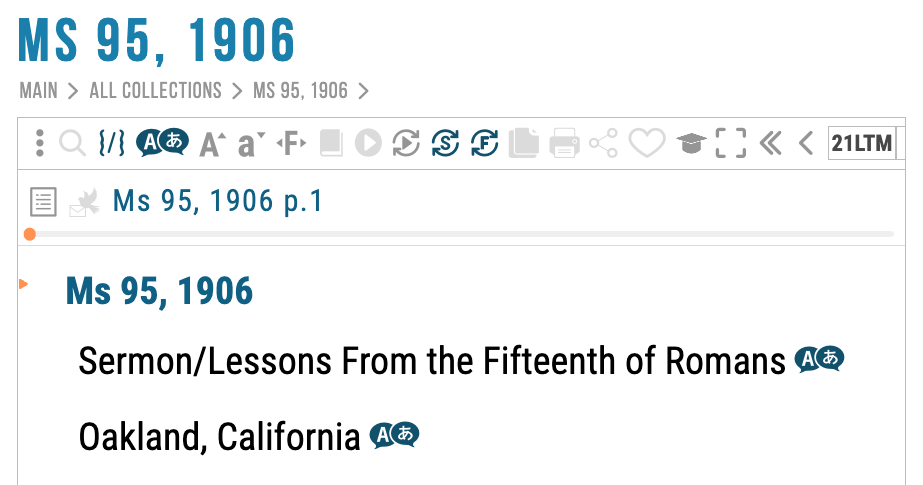
\includegraphics[width=1\linewidth]{images/sermons-and-talks.png}
    \label{fig:enter-label}
\end{figure}


\begin{figure}
    \centering
    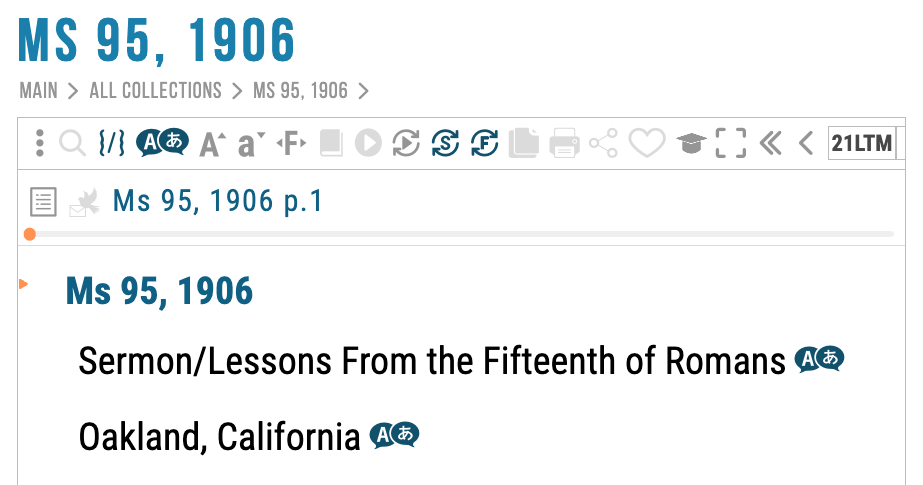
\includegraphics[width=1\linewidth]{images/sermons-and-talks.png}
    \label{fig:enter-label}
\end{figure}


For us, personally, these quotations are unauthenticated and, especially, invalid compared to Ellen White’s authenticated works. But if someone insists on weighing her unconfirmed reports and published writings equally, we will not stand in their way but even further push the conclusion of the Holy Spirit as a being. Let’s follow together.


Kwa sisi, kibinafsi, nukuu hizi hazijathibitishwa na, haswa, ni batili ikilinganishwa na Kazi zilizothibitishwa za Ellen White. Lakini ikiwa mtu anasisitiza kumpima bila kuthibitishwa kwa ripoti na maandishi yaliyochapishwa kwa usawa, hatutasimama katika njia yao lakini hata kusukuma zaidi hitimisho la Roho Mtakatifu kama kiumbe. Tufuate pamoja.


Even compared with Ellen White’s authenticated works, such a Holy Spirit, a being, would not be one with God because Christ was \egwinline{\textbf{The only being who was one with God}}[Lt121-1897.7; 1897][https://egwwritings.org/read?panels=p7266.13]. This Holy Spirit, a being, could not \egwinline{\textbf{enter into all the counsels and purposes of God}}, because Christ was \egwinline{\textbf{the only being}}[PP 34.1; 1890][https://egwwritings.org/read?panels=p84.75] who could do that. This Being is not to be exalted because \egwinline{\textbf{The Father and the Son \underline{alone} are to be exalted}}[YI, July 7, 1898 par.2.; 1898][https://egwwritings.org/read?panels=p469.2964]. The Holy Spirit, as a being, would not fit in the order of heaven as the third being because Satan was \egwinline{\textbf{next to Christ the most exalted \underline{being}} in the heavenly courts}[RH August 9, 1898, par. 7; 1898][https://egwwritings.org/read?panels=p821.17145]. This Holy Spirit, a being, was not invested in the cost of salvation; neither was he in the covenant with Father and Son to save the world, nor dishonored by man’s transgression.


Hata ikilinganishwa na kazi zilizothibitishwa za Ellen White, hiyo Roho Mtakatifu kama, kiumbe, angefanya isiwe kitu kimoja na Mungu kwa sababu Kristo alikuwa \egwinline{\textbf{Nafsi pekee ambaye alikuwa mmoja na Mungu}}[Lt121-1897.7; 1897][https://egwwritings.org/read?panels=p7266.13]. Huyu Roho Mtakatifu, kama nafsi, hakuweza \egwinline{\textbf{kuingia katika mashauri na makusudi yote ya Mungu}}, kwa sababu Kristo alikuwa \egwinline{\textbf{Nafsi pekee}}[PP 34.1; 1890][https://egwwritings.org/read?panels=p84.75] ambaye angeweza kufanya hivyo. Nafsi huyu si wa kuinuliwa kwa sababu \egwinline{\textbf{Baba na Mwana pekee ndio wanaopaswa kuinuliwa}}[YI, July 7, 1898 par.2.; 1898][https://egwwritings.org/read?panels=p469.2964]. Roho Mtakatifu, kama nafsi, hangefanya katika mpangilio wa mbinguni kama Nafsi wa tatu kwa sababu Shetani alikuwa \egwinline{\textbf{aliyetukuka zaidi karibu na Kristo katika nyua za mbinguni}}[RH August 9, 1898, par. 7; 1898][https://egwwritings.org/read?panels=p821.17145]. Huyu Roho Mtakatifu, kiumbe, hakuwekezwa katika gharama ya wokovu; wala hakuwa katika agano na Baba na Mwana kuokoa ulimwengu, wala kudharauliwa na uasi wa mwanadamu.


\egwinline{The great gift of salvation has been placed within our reach at an \textbf{infinite cost to the Father and the Son}.}[RH November 21, 1912, par. 2; 1912][https://egwwritings.org/read?panels=p821.33329]


\egwinline{Kipawa kikuu cha wokovu kimewekwa karibu na uwezo wetu wa kukifikilia kwa gharama isiyo na kikomo kwa Baba na Mwana.}[RH November 21, 1912, par. 2; 1912][https://egwwritings.org/read?panels=p821.33329]


\egwinline{In the plan to save a lost world, the counsel was between them \textbf{\underline{both}}; \textbf{the covenant of peace was between the Father and the Son}.}[ST December 23, 1897, par. 2; 1897][https://egwwritings.org/read?panels=p820.14803]


\egwinline{Katika mpango wa kuokoa ulimwengu uliopotea, shauri lilikuwa kati yao \textbf{\underline{wawili}}; \textbf{agano la amani lilikuwa kati ya Baba na Mwana}.}[ST December 23, 1897, par. 2; 1897][https://egwwritings.org/read?panels=p820.14803]


\egwinline{But in the transgression of man \textbf{\underline{both} the Father and the Son were dishonored}.}[ST December 12, 1895, par. 7; 1895][https://egwwritings.org/read?panels=p820.13243]


\egwinline{Lakini katika kosa la mwanadamu \textbf{\underline{wote} Baba na Mwana walivunjiwa heshima}.}[ST December 12, 1895, par. 7; 1895][https://egwwritings.org/read?panels=p820.13243]


Such a Holy Spirit, a being, does not fit into harmony with the authenticated reports of Ellen White, nor with the Scriptures. The Holy Spirit is called ‘\textit{spirit}’, so it is a spirit, exclusively.


Roho Mtakatifu kama huyo, kiumbe, hapatani na ripoti zilizothibitishwa za Ellen White, wala na Maandiko. Roho Mtakatifu anaitwa ‘\textit{roho}’, kwa hiyo ni roho, pekee.


Many of Sister White’s quotations are sourced from sermons or talks that were published after her death. In what follows, we will present a few that are most often discussed in an effort to prove that Sister White was a trinitarian. We invite everyone to weigh these quotations with her authenticated and published work, those during her lifetime.


Nukuu nyingi za Dada White zimetolewa kutoka kwa mahubiri au mazungumzo ambayo yalichapishwa baada ya kifo chake. Katika yafuatayo, tutawasilisha machache ambayo mara nyingi hujadiliwa katika jitihada za kuthibitisha kwamba Dada White alikuwa mwamini-utatu. Tunakaribisha kila mtu apime nukuu hizi na kazi yake iliyothibitishwa na kuchapishwa, wakati wa uhai wake.


“\textit{And then the golden harps are touched, and the music flows all through the heavenly host, and they fall down and worship the Father and the Son and the Holy Spirit}.”\footnote{\href{https://egwwritings.org/?ref=en_Ms139-1906.32&para=9579.38}{EGW; Ms139-1906.32; 1906}} [Sermon/Thoughts on Matthew 4. Oakland, California July 24, 1906; Previously unpublished.]


“\textit{Halafu vinubi vya dhahabu vinaguswa, na muziki unavuma katika jeshi la mbinguni, nao huanguka chini na kumwabudu Baba na Mwana na Roho Mtakatifu}.”\footnote{\href{https://egwwritings.org/?ref=en_Ms139-1906.32&para=9579.38}{EGW; Ms139-1906.32; 1906}} [Mahubiri/Mawazo juu ya Mathayo 4. Oakland, California Julai 24, 1906; Awali haijachapishwa.]


“\textit{We need to realize that the Holy Spirit, who is as much a person as God is a person, is walking through these grounds.}”\footnote{\href{https://egwwritings.org/?ref=en_Ms66-1899.11&para=6622.19}{EGW; Ms66-1899.11: 1899}} [Talk/Extracts From Talks Given by Mrs. E. G. White at the Opening of College Hall, Avondale, and in the Avondale Church]


“\textit{Tunahitaji kutambua kwamba Roho Mtakatifu, ambaye ni Nafsi kama vile Mungu alivyo Nafsi, anatembea katika viwanja hivi}.”\footnote{\href{https://egwwritings.org/?ref=en_Ms66-1899.11&para=6622.19}{EGW; Ms66-1899.11: 1899}} [Mazungumzo/Dondoo kutoka kwa Mazungumzo Yanayotolewa na Bi. E. G. White katika Ufunguzi wa Ukumbi wa Chuo, Avondale, na katika Kanisa la Avondale]
